\chapter{Convolutional and recurrent neural networks}
\label{ch:sequencemodels}

Next, we will implement models which take the ordering of tokens into
account. These includes \acp{CNN} and \acp{RNN}. In \ac{NLP}, \acp{CNN} can
be considered as a ``\ngram extractor'', which looks at a window of tokens.
However, unlike the count vector approach used above, the CNN extracts
``soft'' \ngrams, utilizing the ability of word embeddings to share
statistical strength between words, and outputting a real-valued number
instead of a boolean yes/no value or an integer count.

\acp{RNN} are theoretically able to detect long range patterns, which is
useful for the tasks at hand. For instance, the ability to connect different
sections of a text and refer back to things that have been mentioned before
can be considered a part of language proficiency.


\section{Experimental setup}

As in the last chapter, models are trained on the test set, and use the
development set as validation data to decide which weights to keep. We keep
the weights that gave the highest macro \FI score over the validation set in
the course of training. The reported metrics are also evaluated on the
development set.

Certain aspects of setup for the new models are different from the models in
the previous chapter, but shared between \ac{CNN} and \ac{RNN} models. These
aspects are described in this section.


\subsection{Input length}

The models in this chapter take as input a document of a predetermined
length. We therefore need to set a fixed number of tokens such that shorter
documents were padded to this length, and longer documents truncated. In
order to decide this, we examined the distribution of document lengths in the
training set. All the subsequent values are rounded to the nearest integer.
First, we found the 95th percentile of document lengths, which turned out to
be 701 tokens. Then, we computed the value $Q_2 + 1.5 \cdot (Q_3 - Q_1)$, or
the median plus 1.5 times the interquartile range, which gives 693 tokens.
Finally, we computed the mean value plus two standard deviations, giving 707
tokens. These values are all close to each other, and we decided to settle on
700 tokens since it is a round number close to all values we examined.

As a consequence of the unequal distributions of length between the two test
levels, the documents that are truncated are mainly from the advanced level
test. Thus, the presence of padding tokens at the end is a strong indicator
of a text coming from the AL test. It is potentially problematic that this
truncation only happens to documents from one test level, since the two test
levels are seen to have different distributions of both CEFR scores and
\acp{L1}. Nevertheless, even if truncation did not happen, a model might be
able to discern the test levels just by document length, since we do not hide
the document length from the model.


\subsection{Pre-trained embeddings}
\label{subseq:fasttext}

We experimented with randomly initialized word embedding vectors trained from
scratch, as well as initializing the vectors with pre-trained embeddings. We
know that our corpus contains tokens with spelling mistakes, which are likely
to be absent in any pre-trained vector model. We therefore sought out
pre-trained models using the FastText algorithm, which lets us compute
vectors even for words that do not have separate entries in the model, in
which case the model creates a vector based on the word's constituent
character \ngrams.

In our case, we used a selection of models trained on a large Norwegian
corpus, the combination of Norsk aviskorpus (The Norwegian Newspaper Corpus)
and NoWaC (Norwegian Web As Corpus) \autocite{stadsnes2018}. These vector
models are very large, containing vectors for more than 2,500,000 words. The
models are stored in a repository that is available online and on the Abel
supercomputer cluster \autocite{murhaf2017repository}. We use three models
trained on this corpus using the FastText algorithm, differing only in the
dimension of embeddings. They were trained using skipgram and window size 5, 
and lemmatization has not been applied to the corpora.

We can superficially confirm the usefulness of FastText embeddings by looking
at vector similarities. We use the Python library Gensim \autocite{gensim} to
load vector models and look up word similarities. For instance, the token
`kjokoladet' is a misspelt version of `sjokolade' (chocolate), and it is
closest in the embedding space to `sjokolade'. Curiously, it is also closer
to `potetgul' than `potetgull' (potato crisps), and the former is a
misspelling.

Our training data only contains 20,766 unique tokens, which is less than 1\%
of the full vocabulary of the models. Loading the full pre-trained model
takes a long time and uses huge amounts of memory for word vectors we will
never use. For that reason, we created models of smaller size by loading the
full models once and iterating through all of the word forms in our corpus,
storing the resulting vectors in a new vector model containing only 20,766
words. In this way, we are also able to benefit from the FastText models'
ability to compute vectors for unknown words, since the \ngram algorithm is
being used when computing the reduced models. However, after the embedding
layers of our models have been initialized with vectors from the fastText
model, fine-tuning of vectors happens in the same way as if we had used
embeddings from any other model such as Word2vec, or even randomly
initialized embeddings, since the FastText network is not incorporated into
our models.

Two common variations on training a neural model with pre-trained word
embeddings are using dynamic embeddings, where the embedding vectors are
updated by gradient descent as part of training the entire network, and
static embeddings, where the embedding vectors are kept constant while other
weights in the network are updated. Additional variations are also found in
literature, for example the multi-channel approach seen in
\textcite{kim2014convolutional} where two embedding layers, one static and
one dynamic, are run in parallel.

We will use both static and dynamic embeddings in our experiments, but not in
a multi-channel setup. For RNN experiments, we will limit our experiments to
dynamic word embeddings only.

Experiments using mixed UPOS tags as input will not use pre-trained
embeddings. This is because of two reasons. First, we do not have any
pre-trained embeddings for UPOS tags. Second, the pre-trained word embeddings
for function words that occur in the mixed UPOS tag representation are
trained in the context of content words, and we therefore do not expect them
to have much utility in the context of UPOS tags.


\subsection{Multi-channel input}

In some of our experiments we use both word tokens and their POS tags as
input at the same time. To do this we include two separate embedding matrices
in our network, one for words and one for POS tags. These embedding matrices
do not have to be of the same dimensions, and since the number of different
POS tags is very low compared to the number of different words, we use
smaller vectors for POS tags.

To create the input to the core part of our network, we concatenate the word
and POS embeddings into a single vector. For instance, if we use word
embeddings of size 100 and POS embeddings of size 10, the next layer will
receive vectors of size 110.


\section{Convolutional neural networks}

We create a model with a convolutional architecture based on the model
described in \textcite{kim2014convolutional}. Documents are represented as
sequences of token IDs, and fed into an embedding lookup layer. A separate
token ID is used for padding if the document is shorter than 700 tokens.
Another unique token ID is used for unknown tokens, i.e. tokens that either
are not present in training data, or are not among the $n$ most frequent
tokens, if we select a frequency cutoff.

The central part of the architecture is a set of convolutional filter banks
that are applied to sequences of embeddings. We may use several different
window sizes for the filters. The default architecture from
\textcite{kim2014convolutional} uses 300 convolutional filters: 100 each of
window size 3, 4 and 5. After applying the convolutions, the output is max
pooled along the time axis. This selects the highest output each filter
computed across all windows in the document. In practice, three pooling
operations are included in the computational graph, one for each filter bank.
This is a technical consideration, necessary because of the different window
sizes.

The pooled vectors for each of the filter banks are concatenated into a
single vector, representing the document as a whole. This vector has as many
elements as there are filters in all the filter banks combined. This
representation vector is fed to a final softmax layer to produce a
classification output. During training, we apply dropout to this final weight
layer as a regularization method.


\subsection{Results}

The \ac{CNN} classifier that used both tokens and POS tags as input performed
better than the one which only used tokens as input, as seen in table
\ref{tab:cnn-results}. However, on the collapsed label set, the model which
only used tokens had a higher accuracy. Filters of size 3, 4, and 5 were
used. The last dense layer uses dropout with $p=0.5$ and a constraint on
maximum $L_2$ norm of 3.

\begin{table}
  \centering
  \begin{tabular}{lrrrr}
    \toprule
      & \multicolumn{2}{c}{All labels}   & \multicolumn{2}{c}{Collapsed labels} \\
    \cmidrule(lr){2-3}
    \cmidrule(lr){4-5}
    Model   & Macro \FI   & Micro \FI   & Macro \FI   & Micro \FI \\
    \midrule
    \multicolumn{5}{c}{Randomly initialized embeddings} \\
    \midrule
    % $BEGIN autotable cnn-results
    % $META models-per-row=2 columns-per-model=macrof1,microf1
    % $ROW CNN:             cnn-26515464_1    cnn-26518498_1
    % $ROW CNN+POS:         cnn-26515464_2    cnn-26518498_2
    % $ROW CNN Mix:         cnn-26515464_3    cnn-26518498_3
    % $ROW CNN Reg:         cnn-26515464_4    cnn-26518498_4
    % $ROW CNN Reg+POS:     cnn-26515464_5    cnn-26518498_5
    % $ROW CNN Reg Mix:     cnn-26515464_6    cnn-26518498_6
    % $ROW CNN Rank:        cnn-26515464_7    cnn-26518498_7
    % $ROW CNN Rank+POS:    cnn-26515464_8    cnn-26518498_8
    % $ROW CNN Rank Mix:    cnn-26515464_9    cnn-26518498_9
    %\midrule \multicolumn{5}{c}{Pre-trained, fine tuned embeddings} \\ \midrule
    % $ROW CNN:             cnn-26515464_10   cnn-26518498_10
    % $ROW CNN+POS:         cnn-26515464_11   cnn-26518498_11
    % $ROW CNN Reg:         cnn-26515464_13   cnn-26518498_12
    % $ROW CNN Reg+POS:     cnn-26515464_14   cnn-26518498_13
    % $ROW CNN Rank:        cnn-26515464_16   cnn-26518498_14
    % $ROW CNN Rank+POS:    cnn-26515464_17   cnn-26518498_15
    % $END autotable
    CNN & $0.168$ & $\mathbf{0.398}$ & $0.388$ & $0.732$ \\
    CNN+POS & $0.146$ & $0.374$ & $0.398$ & $0.748$ \\
    CNN Mix & $0.201$ & $\mathbf{0.398}$ & $0.383$ & $0.724$ \\
    CNN Reg & $0.230$ & $0.382$ & $0.439$ & $0.724$ \\
    CNN Reg+POS & $0.236$ & $0.341$ & $0.383$ & $0.724$ \\
    CNN Reg Mix & $\mathbf{0.258}$ & $\mathbf{0.398}$ & $0.412$ & $0.642$ \\
    CNN Rank & $0.177$ & $0.374$ & $0.392$ & $0.740$ \\
    CNN Rank+POS & $0.187$ & $0.382$ & $0.397$ & $0.748$ \\
    CNN Rank Mix & $0.231$ & $0.382$ & $0.379$ & $0.715$ \\
    \midrule
    \multicolumn{5}{c}{Pre-trained, fine tuned embeddings} \\
    \midrule
    CNN & $0.208$ & $0.382$ & $0.384$ & $0.724$ \\
    CNN+POS & $0.161$ & $0.366$ & $0.402$ & $\mathbf{0.756}$ \\
    CNN Reg & $0.242$ & $0.341$ & $\mathbf{0.463}$ & $0.724$ \\
    CNN Reg+POS & $0.232$ & $0.366$ & $0.411$ & $0.715$ \\
    CNN Rank & $0.198$ & $0.350$ & $0.384$ & $0.724$ \\
    CNN Rank+POS & $0.181$ & $0.325$ & $0.401$ & $\mathbf{0.756}$ \\
    \bottomrule
  \end{tabular}
  \caption[\FI scores of CNN classifiers on AES.]{
    \FI scores of CNN classifiers on AES. +POS: Multi-channel input with
    both words and UPOS tags. Reg: Regression model. Rank: Ordinal regression.
  }
  \label{tab:cnn-results}
\end{table}


\subsubsection{Effect of hyperparameters}

Comparing the different prediction methods, namely categorical
classification, numeric regression and ordinal regression, we see that
numeric regression overall has the highest macro \FI scores. This is similar
to the observations we made in the previous chapter. Based on this, we
decided to stick to neural regression models only in the next section, where
we train \ac{RNN} models.


\subsection{Training behaviour}

\begin{figure}
  % cnn-26515464_6
  \begin{subfigure}{\linewidth}
    \centering
    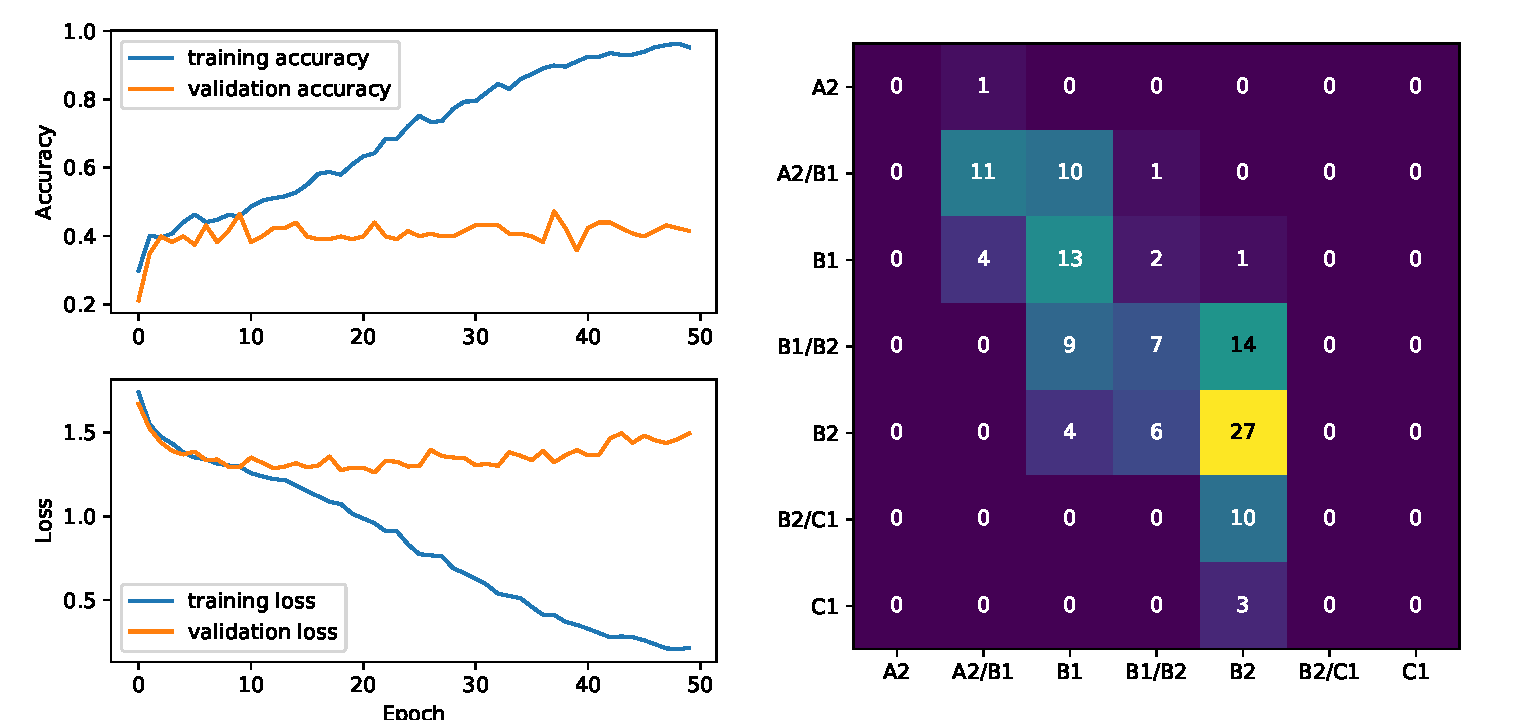
\includegraphics{cnn-training}
    \caption{
      Training and validation loss and validation F1 over 50 epochs of
      training.
    }
  \end{subfigure}
  \begin{subfigure}{\linewidth}
    \centering
    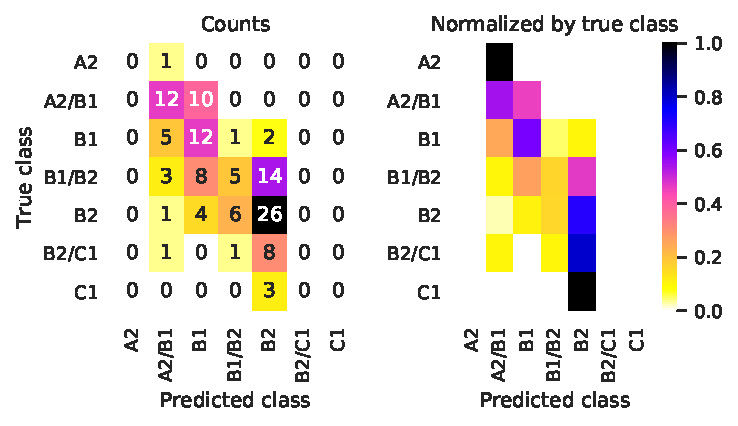
\includegraphics{cnn-confusion}
    \caption{
      Confusion matrix on validation set, raw counts and normalized.
    }
  \end{subfigure}
  \caption[Training behaviour of CNN regression]{
    CNN regressor with mixed UPOS tags as input.
  }
  \label{fig:cnn-training}
\end{figure}

Figure \ref{fig:cnn-training} shows that how the training and validation
metrics evolve in the course of training, as well as the confusion matrix of
the final model. While the training loss quickly converges to a very low
value, the validation loss fluctuates around a much higher loss, indicating
overfitting. The plot of validation macro \FI also shows large fluctuations.

The confusion matrix reveals that the final model did not assign any samples
to the classes `A2', and `C1', the peripheral classes which are also the
smallest in the validation set. As noted in the discussion about metrics in
the previous chapter (\ref{metrics-discussion}), classes with no predictions
contribute to a low macro \FI score.

Overall, the convolutional models were not able to improve on the macro or
micro \FI scores the \ac{MLP} models in the previous chapter achieved.
However, while the \ac{MLP} confusion matrix (fig. \ref{fig:mlp-char-rank})
had several predictions scattered away from the diagonal, the confusion
matrix for the \ac{CNN} looks like a fuzzy diagonal line, with gradual
dropoff as the distance from the diagonal increases. It also looks like it
has a steeper slope than the ideal diagonal running between the top-left and
bottom-right corner, which is not ideal, but even if the slope is wrong, a
diagonal indicates that relative ranks between essays are reasonable.

We wondered whether the visible difference between scattered predictions and
a fuzzy diagonal could be explained using other metrics than macro or micro
\FI, on which we have previously decided to base our model evaluations. As
seen in table \ref{tab:mlp-cnn-metrics}, while the \ac{MLP} has the best \FI
scores, the \ac{CNN} beats it in terms of ranking and error metrics. This
explains the intuition of the CNN confusion matrix looking better.

It is worth noting that CNN Reg Mix has 149,101 trainable parameters, compared
to the 2,032,206 of MLP Rank char, which is more than 13 times as many.

\begin{table}
  \centering
  \begin{tabular}{lrr}
    \toprule
    Metric                       & MLP Rank Char & CNN Reg Mix \\
    \midrule
    Macro \FI                     & $\mathbf{0.330}$ & $0.258$ \\
    Micro \FI                     & $\mathbf{0.480}$ & $0.398$ \\
    Spearman's ranked correlation & $0.580$ & $\mathbf{0.647}$ \\
    Mean absolute error           & $0.805$ & $\mathbf{0.756}$ \\
    Root mean squared error       & $1.24$  & $\mathbf{1.03}$ \\
    \bottomrule
  \end{tabular}
  \caption[Comparison of metrics for a MLP and a CNN model]{
    Metrics for MLP Rank Char and CNN Reg Mix. For error metrics, lower values
    are better.
  }
  \label{tab:mlp-cnn-metrics}
\end{table}



\section{Recurrent neural networks}

Next, we moved to a different kind of architecture, \acp{RNN}. We implemented
several models that were variants of the architecture described in
\textcite{taghipour16}. The various changes we made to their architecture
are described below. Some of our variations are similar to the variations
in \textcite{taghipour16}, while others are different ideas. There are also
variations from the paper that we do not implement ourselves, such as a
combined \ac{RNN} and \ac{CNN} model.

were made in order to accommodate our data \todo{which?}. 

We explore some variations in hyperparameters, namely LSTM vs. GRU cells,
unidirectional networks vs. BiRNN, different input representations, different
pooling methods, and compare random initialization of the embedding layer
with using pre-trained vectors.

The embedding layer in \textcite{taghipour16} was of dimension 50 and
randomly initialized. We increased the embedding dimension to 100, and
experiment both with randomly initialized embeddings and with pre-trained
ones.

We are reporting macro and micro \FI as before, not QWK as
\citeauthor{taghipour16}. Refer to section \ref{metrics-discussion} for the
discussion of different metrics for the task.

The ASAP data that \citeauthor{taghipour16} use consists of essays from eight
different prompts, and the range of scores differs across prompts. Since the
scores are numeric values over different ranges, modelling the task as a
regression problem made it sufficient to normalize the numeric scores to a
common interval before training.

Unlike our corpus, ASK, the ASAP dataset used by \citeauthor{taghipour16}
contained essays that were not necessarily written in a second language. Our
data is not split into different parts based on the prompt. There are two
different test levels in ASK, but these are not distinguished in training.


\subsection{Variants}

We create \acp{RNN} with two different types of gated \ac{RNN} cell, the
\ac{LSTM} and the \ac{GRU}. The concept of gated cells is explained in
section \ref{seq:rnn}, along with the equations defining the gated cells. In
Keras, the default activation function for the gates in gated RNNs is the
\emph{Hard sigmoid} activation function (ref. eq. \ref{eq:hardsigmoid}),
chosen because it is computationally more efficient than the sigmoid
function.

We attempted three different pooling methods, that is, ways of combining a
sequence of hidden states from the \ac{RNN} into a feature vector. The first
approach is \emph{mean over time}, where we apply element-wise, unweighted
averaging to the RNN output across the time dimension. This means that the
first element of the representation vector is the average of the first
element of the RNN output across time, and similarly for the second element,
etc., as in the following equation:

\[
  \mathrm{mean/time}(x_i) = \frac{1}{T}\sum_{t=0}^T o_{t,i}
\]

where $T$ is the total number of time steps, and $o_{t,i}$ is the output of
the RNN at time step $t$ and index $i$.

The second method is similar to the first, except that the averaging
operation is replaced by a max operation. Each dimension of the vector is the
highest value the hidden state had at that dimension across the entire
sequence. We refer to this as the \emph{max over time}, and it is defined by
the following equation:

\[
  \mathrm{max/time}(x_i) = \max_{t=0}^T o_{t,i}
\]

The final method we used is an attention layer, which differs from the mean
over time layer in that time steps are weighted by an attention mechanism: a
single-layer neural network computes a value between -1 and 1 for each time
step. These values are normalized across all time steps by a softmax layer,
and then used to compute the weighted average.

Since each time step contributes to the final representation in differing
amounts, the mechanism should be able in theory to focus on crucial
information by choosing weights such as to disregard uninformative time
steps, improving performance. The attention mechanism is trained along with
the rest of the network.

The bidirectional models (BiRNN) are constructed by running two \acp{RNN}
over the same input, but in opposite directions. The output from the BiRNN
layer is a sequence of vectors where, for each time step $j$, the vector is
the concatenation of two vectors $[s_f;s_b]$ where $s_f$ at time step $j$ is
the output from the forwards \ac{RNN} after processing the inputs $(x_1, x_2,
\ldots, x_j)$ and $s_b$ the output from the backwards \ac{RNN} after
processing the inputs $(x_m, x_{m-1}, \ldots, x_j)$, where $m$ is the total
number of time steps. The BiRNN should therefore be able to extract context
on both sides of a input time step.

All the models have a hidden state vector of size 300 in unidirectional
\acp{RNN}, and 600 in BiRNNs (300 in each direction). We use all tokens in
the training set as our lexicon, giving a vocabulary size of 20,068 (20,066
unique tokens occurring in the training set, plus two tokens for padding and
unknown words). This entails that the unknown token will receive no training
signal, and remain whatever it was initialized as, which is either a random
vector or the embedding computed by the fastText model for the token
`\_\_UNK\_\_'. \todo{sanity}

Embeddings are initialized either randomly or using vectors
from the fastText model described in section \ref{subseq:fasttext}, and
trained as part of the network. BiRNNs are referred to in the following
tables and discussion as either BiLSTM or BiGRU, depending on the RNN cell
used.


\section{Results}

The RNN results are split into two tables. Table \ref{tab:lstm-results}
contains the results for models with \ac{LSTM} cells, while table
\ref{tab:gru-results} contains the results for models with \ac{GRU} cells.
The mixed input format is only listed in the sections with randomly
initialized embeddings, as it is not applicable when using pre-trained
embeddings.

\begin{table}
  \centering
  \begin{tabular}{lrrrr}
    \toprule
            & \multicolumn{2}{c}{All labels} & \multicolumn{2}{c}{Collapsed labels} \\
    \cmidrule(lr){2-3}
    \cmidrule(lr){4-5}
    Model     & Macro \FI      & Micro \FI      & Macro \FI      & Micro \FI \\
    \midrule
              \multicolumn{5}{c}{Random init, unidirectional LSTM} \\
    \midrule
    % $BEGIN autotable lstm-results
    % $META models-per-row=2 columns-per-model=macrof1,microf1
    % $ROW Mean:        rnn-26519203_1       rnn-26519204_1
    % $ROW Max:         rnn-26519203_2       rnn-26519204_2
    % $ROW Attn.:        rnn-26519203_3       rnn-26519204_3
    % $ROW +POS Mean:   rnn-26519203_4       rnn-26519204_4
    % $ROW +POS Max:    rnn-26519203_5       rnn-26519204_5
    % $ROW +POS Attn:   rnn-26519203_6       rnn-26519204_6
    % $ROW Mix Mean:    rnn-26519203_7       rnn-26519204_7
    % $ROW Mix Max:     rnn-26519203_8       rnn-26519204_8
    % $ROW Mix Attn:    rnn-26519203_9       rnn-26519204_9
    % \midrule \multicolumn{5}{c}{Random init, BiLSTM} \\ \midrule
    % $ROW Mean:        rnn-26530015_10      rnn-26530016_10
    % $ROW Max:         rnn-26530015_11      rnn-26530016_11
    % $ROW Attn:        rnn-26530015_12      rnn-26530016_12
    % $ROW +POS Mean:   rnn-26530015_13      rnn-26530016_13
    % $ROW +POS Max:    rnn-26530015_14      rnn-26530016_14
    % $ROW +POS Attn:   rnn-26530015_15      rnn-26530016_15
    % $ROW Mix Mean:    rnn-26530015_16      rnn-26530016_16
    % $ROW Mix Max:     rnn-26530015_17      rnn-26530016_17
    % $ROW Mix Attn:    rnn-26530015_18      rnn-26530016_18
    % \midrule \multicolumn{5}{c}{Pre-trained, unidirectional LSTM} \\ \midrule
    % $ROW Mean:        rnn-26519203_19      rnn-26519204_19
    % $ROW Max:         rnn-26519203_20      rnn-26519204_20
    % $ROW Attn:        rnn-26519203_21      rnn-26519204_21
    % $ROW +POS Mean:   rnn-26519203_22      rnn-26519204_22
    % $ROW +POS Max:    rnn-26519203_23      rnn-26519204_23
    % $ROW +POS Attn:   rnn-26519203_24      rnn-26519204_24
    % \midrule \multicolumn{5}{c}{Pre-trained, BiLSTM} \\ \midrule
    % $ROW Mean:        rnn-26530015_25      rnn-26530016_25
    % $ROW Max:         rnn-26530015_26      rnn-26530016_26
    % $ROW Attn:        rnn-26530015_27      rnn-26530016_27
    % $ROW +POS Mean:   rnn-26530015_28      rnn-26530016_28
    % $ROW +POS Max:    rnn-26530015_29      rnn-26530016_29
    % $ROW +POS Attn:   rnn-26530015_30      rnn-26530016_30
    % $END autotable
    Mean & $0.268$ & $0.398$ & $0.458$ & $0.675$ \\
    Max & $0.235$ & $0.350$ & $0.475$ & $0.740$ \\
    Attn. & $0.445$ & $0.431$ & $0.624$ & $0.780$ \\
    +POS Mean & $0.251$ & $0.358$ & $0.454$ & $0.699$ \\
    +POS Max & $0.187$ & $0.325$ & $0.435$ & $0.715$ \\
    +POS Attn & $0.417$ & $0.390$ & $0.619$ & $0.772$ \\
    Mix Mean & $0.230$ & $0.350$ & $0.396$ & $0.626$ \\
    Mix Max & $0.210$ & $0.415$ & $0.398$ & $0.748$ \\
    Mix Attn & $0.297$ & $0.431$ & $0.576$ & $0.772$ \\
    \midrule \multicolumn{5}{c}{Random init, BiLSTM} \\ \midrule
    Mean & $0.262$ & $0.366$ & $0.457$ & $0.699$ \\
    Max & $0.182$ & $0.358$ & $0.485$ & $0.724$ \\
    Attn & $\mathbf{0.448}$ & $0.447$ & $0.699$ & $0.805$ \\
    +POS Mean & $0.337$ & $0.333$ & $0.441$ & $0.691$ \\
    +POS Max & $0.176$ & $0.350$ & $0.460$ & $0.715$ \\
    +POS Attn & $0.420$ & $0.407$ & $0.670$ & $0.789$ \\
    Mix Mean & $0.220$ & $0.309$ & $0.402$ & $0.659$ \\
    Mix Max & $0.190$ & $0.374$ & $0.400$ & $0.756$ \\
    Mix Attn & $0.305$ & $0.447$ & $0.550$ & $0.724$ \\
    \midrule \multicolumn{5}{c}{Pre-trained, unidirectional LSTM} \\ \midrule
    Mean & $0.266$ & $0.374$ & $0.443$ & $0.675$ \\
    Max & $0.181$ & $0.358$ & $0.433$ & $0.756$ \\
    Attn & $0.410$ & $0.423$ & $0.626$ & $0.789$ \\
    +POS Mean & $0.280$ & $0.390$ & $0.465$ & $0.691$ \\
    +POS Max & $0.206$ & $0.415$ & $0.414$ & $0.780$ \\
    +POS Attn & $0.370$ & $0.382$ & $0.680$ & $\mathbf{0.813}$ \\
    \midrule \multicolumn{5}{c}{Pre-trained, BiLSTM} \\ \midrule
    Mean & $0.263$ & $0.374$ & $0.470$ & $0.683$ \\
    Max & $0.190$ & $0.325$ & $0.396$ & $0.748$ \\
    Attn & $0.429$ & $\mathbf{0.463}$ & $0.638$ & $0.805$ \\
    +POS Mean & $0.257$ & $0.350$ & $0.465$ & $0.691$ \\
    +POS Max & $0.181$ & $0.358$ & $0.412$ & $0.715$ \\
    +POS Attn & $0.427$ & $0.423$ & $\mathbf{0.704}$ & $0.780$ \\
    \bottomrule
  \end{tabular}
  \caption{\FI scores of LSTM classifiers on AES}
  \label{tab:lstm-results}
\end{table}

\begin{table}
  \centering
  \begin{tabular}{lrrrr}
    \toprule
            & \multicolumn{2}{c}{All labels} & \multicolumn{2}{c}{Collapsed labels} \\
    \cmidrule(lr){2-3}
    \cmidrule(lr){4-5}
    Model     & Macro \FI      & Micro \FI      & Macro \FI      & Micro \FI \\
    \midrule
              \multicolumn{5}{c}{Random init, unidirectional GRU} \\
    \midrule
    % $BEGIN autotable gru-results
    % $META models-per-row=2 columns-per-model=macrof1,microf1
    % $ROW Mean:        rnn-26536430_1       rnn-26536431_1
    % $ROW Max:         rnn-26536430_2       rnn-26536431_2
    % $ROW Attn:        rnn-26536430_3       rnn-26536431_3
    % $ROW +POS Mean:   rnn-26536430_4       rnn-26536431_4
    % $ROW +POS Max:    rnn-26536430_5       rnn-26536431_5
    % $ROW +POS Attn:   rnn-26536430_6       rnn-26536431_6
    % $ROW Mix Mean:    rnn-26536430_7       rnn-26536431_7
    % $ROW Mix Max:     rnn-26536430_8       rnn-26536431_8
    % $ROW Mix Attn:    rnn-26536430_9       rnn-26536431_9
    % \midrule \multicolumn{5}{c}{Random init, BiGRU} \\ \midrule
    % $ROW Mean:        rnn-26536430_10      rnn-26536431_10
    % $ROW Max:         rnn-26536430_11      rnn-26536431_11
    % $ROW Attn:        rnn-26536430_12      rnn-26536431_12
    % $ROW +POS Mean:   rnn-26536430_13      rnn-26536431_13
    % $ROW +POS Max:    rnn-26536430_14      rnn-26536431_14
    % $ROW +POS Attn:   rnn-26536430_15      rnn-26536431_15
    % $ROW Mix Mean:    rnn-26536430_16      rnn-26536431_16
    % $ROW Mix Max:     rnn-26536430_17      rnn-26536431_17
    % $ROW Mix Attn:    rnn-26536430_18      rnn-26536431_18
    % \midrule \multicolumn{5}{c}{Pre-trained, unidirectional GRU} \\ \midrule
    % $ROW Mean:        rnn-26536430_19      rnn-26536431_19
    % $ROW Max:         rnn-26536430_20      rnn-26536431_20
    % $ROW Attn:        rnn-26536430_21      rnn-26536431_21
    % $ROW +POS Mean:   rnn-26536430_22      rnn-26536431_22
    % $ROW +POS Max:    rnn-26536430_23      rnn-26536431_23
    % $ROW +POS Attn:   rnn-26536430_24      rnn-26536431_24
    % \midrule \multicolumn{5}{c}{Pre-trained, BiGRU} \\ \midrule
    % $ROW Mean:        rnn-26536430_25      rnn-26536431_25
    % $ROW Max:         rnn-26536430_26      rnn-26536431_26
    % $ROW Attn:        rnn-26536430_27      rnn-26536431_27
    % $ROW +POS Mean:   rnn-26536430_28      rnn-26536431_28
    % $ROW +POS Max:    rnn-26536430_29      rnn-26536431_29
    % $ROW +POS Attn:   rnn-26536430_30      rnn-26536431_30
    % $END autotable
    Mean & $0.264$ & $0.374$ & $0.455$ & $0.675$ \\
    Max & $0.219$ & $0.325$ & $0.487$ & $0.683$ \\
    Attn & $0.434$ & $0.431$ & $\mathbf{0.806}$ & $0.805$ \\
    +POS Mean & $0.348$ & $0.398$ & $0.450$ & $0.642$ \\
    +POS Max & $0.230$ & $0.374$ & $0.500$ & $0.748$ \\
    +POS Attn & $0.434$ & $0.423$ & $0.718$ & $0.813$ \\
    Mix Mean & $0.225$ & $0.333$ & $0.388$ & $0.634$ \\
    Mix Max & $0.200$ & $0.398$ & $0.398$ & $0.756$ \\
    Mix Attn & $0.302$ & $\mathbf{0.455}$ & $0.509$ & $0.780$ \\
    \midrule \multicolumn{5}{c}{Random init, BiGRU} \\ \midrule
    Mean & $0.314$ & $0.333$ & $0.444$ & $0.667$ \\
    Max & $0.160$ & $0.325$ & $0.460$ & $0.691$ \\
    Attn & $0.459$ & $0.447$ & $0.805$ & $0.805$ \\
    +POS Mean & $0.373$ & $0.333$ & $0.425$ & $0.683$ \\
    +POS Max & $0.175$ & $0.309$ & $0.503$ & $0.748$ \\
    +POS Attn & $\mathbf{0.460}$ & $0.447$ & $0.687$ & $\mathbf{0.821}$ \\
    Mix Mean & $0.231$ & $0.350$ & $0.395$ & $0.642$ \\
    Mix Max & $0.200$ & $0.382$ & $0.405$ & $0.764$ \\
    Mix Attn & $0.275$ & $\mathbf{0.455}$ & $0.617$ & $0.707$ \\
    \midrule \multicolumn{5}{c}{Pre-trained, unidirectional GRU} \\ \midrule
    Mean & $0.274$ & $0.366$ & $0.463$ & $0.715$ \\
    Max & $0.185$ & $0.350$ & $0.401$ & $0.756$ \\
    Attn & $0.414$ & $0.431$ & $0.678$ & $0.797$ \\
    +POS Mean & $0.282$ & $0.382$ & $0.477$ & $0.699$ \\
    +POS Max & $0.193$ & $0.382$ & $0.405$ & $0.764$ \\
    +POS Attn & $0.409$ & $0.423$ & $0.746$ & $0.789$ \\
    \midrule \multicolumn{5}{c}{Pre-trained, BiGRU} \\ \midrule
    Mean & $0.266$ & $0.390$ & $0.435$ & $0.707$ \\
    Max & $0.187$ & $0.398$ & $0.393$ & $0.740$ \\
    Attn & $0.454$ & $0.447$ & $0.773$ & $0.797$ \\
    +POS Mean & $0.281$ & $0.382$ & $0.480$ & $0.724$ \\
    +POS Max & $0.183$ & $0.341$ & $0.397$ & $0.748$ \\
    +POS Attn & $0.433$ & $0.439$ & $0.758$ & $0.805$ \\
    \bottomrule
  \end{tabular}
  \caption{\FI scores of GRU classifiers on AES}
  \label{tab:gru-results}
\end{table}


\subsection{The effect of hyperparameters}

\todo{expand}
We choose five different hyperparameters and examine the effect each of them
has on the predictions of the networks. When it is relevant, we will compare
the effect we got with the effect found by \textcite{taghipour16}. However,
our experiments are not directly comparable, for reasons including different
evaluation metric, and different evaluation method (\citeauthor{taghipour16}
use 5-fold cross validation).


\subsubsection*{LSTM versus GRU}

GRU comes out on top with somewhat higher macro \FI scores. When ranking all
models by macro \FI score on the full set of labels, the top three places are
taken by GRU models ($0.460$, $0.459$, $0.454$), and the fourth and fifth
places by LSTM models ($0.448$, $0.445$). A GRU model also has the highest
macro \FI on the collapsed labels ($0.805$). The best LSTM macro \FI on
collapsed labels is $0.704$, ranking seventh among all GRU and LSTM
experiments.

We conclude that GRU performs best on the task. An additional benefit of GRU
is that it has fewer parameters and is a little faster in training.


\subsubsection*{Bidirectional RNN}

Our top performing models are BiRNNs, and the unidirectional model with the
highest macro \FI on the full set of labels only ranks fifth among all RNN
experiments (macro \FI $0.445$). When comparing models that differ only in
whether they are bidirectional or not, we do not always see that the macro
\FI is higher in the bidirectional model. However, if we only look at the
models which use an attention mechanism, the bidirectional models win in all
but one case. The GRU attention model with mixed UPOS input drops from
$0.320$ to $0.275$. It seems that BiRNNs may be most effective in conjunction
with an attention mechanism, at least on this dataset.


\subsubsection*{Initialization of embeddings}

The effects of initialization is not very clear, and in any case mixed. The
best LSTM models used pre-trained embeddings, and the best GRU models used
randomly initialized embeddings. However, the best GRU model with pre-trained
embeddings has a higher macro \FI score than the overall best LSTM model,
$0.454$ and $0.448$ respectively.


\subsubsection*{Pooling method}

There are clear differences in the performance of the three pooling method we
have used, mean-over-time, max-over-time and attention. The one that gives
the worst results is max-over-time, which is the only method that ever gives
a macro \FI score less than $0.2$ on the full set of labels, and even the
best run using max pooling has a macro \FI of $0.235$, lower than several CNN
and MLP models trained previously.

Attention comes out as the clear winner of the three pooling methods. It is
the only pooling method that gives macro \FI scores above 40\% in the full
set of classes. At the other end of the scale, max pooling performs worse
than the other two mechanisms in almost every case. Intuitively, it seems
reasonable that max pooling performs poorly on the task. A couple of mistakes
should not count more towards the result than an otherwise consistent level.

The mean-over-time pooling method is somewhere in between, usually giving
macro \FI scores higher than max-over-time and lower than attention.
Interestingly, this is the opposite of what \textcite{taghipour16} found,
even though we are using a very similar network architecture for the same
kind of task. In their case, mean-over-time gave slightly better results than
attention when they compared them (according to the QWK metric).

It can seem promising that the attention mechanism performs well, since it by
design might be able to give more interpretable results than other neural
methods. However, as we will see below (section \ref{subsec:attentionvis}),
it is not apparent that the attention mechanism aids model interpretation in
our case.


\subsubsection*{UPOS tags}

The addition of UPOS tags as a side input seems to have variable effect on
the performance. In the LSTM experiments, all the models with an attention
mechanism had a drop in performance when adding the UPOS side input. However,
in the GRU experiments, some models increased their macro \FI when they used
the UPOS side input, including the overall best model, which had a macro \FI
of $0.459$ without UPOS tags and $0.460$ with them. We also see inconsistent
effects when looking at the results on the collapsed labels.

The mixed UPOS input does not measure up in the RNN context, even though it
had the best results in the CNN experiments. The highest macro \FI from an
RNN with mixed UPOS input is $0.305$ on the full set of labels, and $0.617$
on the collapsed set of labels. This is higher than the best results in the
CNN experiments ($0.258$ and $0.463$). It is possible that RNNs are better
able to make use of the greater amount of information present in full lexical
features.


\subsection{Training behaviour}

\begin{figure}
  % rnn-26536430_15
  \begin{subfigure}{\linewidth}
    \centering
    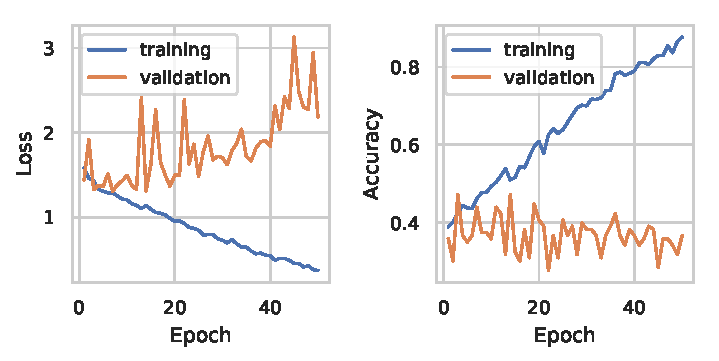
\includegraphics{rnn-training}
    \caption{Training and validation loss and accuracy over 50 epochs of training.}
  \end{subfigure}
  \begin{subfigure}{\linewidth}
    \centering
    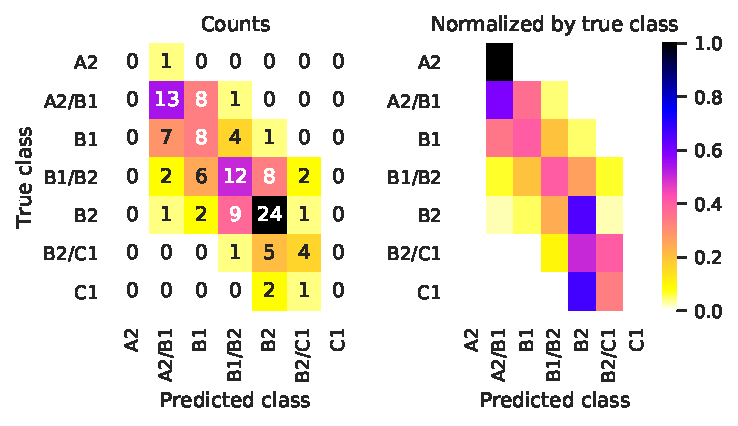
\includegraphics{rnn-confusion}
    \caption{Confusion matrix on validation set, raw counts and normalized.}
  \end{subfigure}
  \caption[Training behaviour of BiGRU with attention]{
    BiRNN with GRU cells, attention mechanism, and pre-trained
    embeddings of dimension 100, fine-tuned.
  }
  \label{fig:rnn-training}
\end{figure}

We see the training and classification of one of the best RNN model in figure
\ref{fig:rnn-training}, a BiGRU model with randomly initialized embeddings
using and an attention mechanism. The plot of the loss shows that the
training loss drops quickly at the beginning and then asymptotically
approaches zero. At the same time, the validation loss quickly converges
around a stable value, but fluctuates somewhat. The plot of macro \FI is more
noisy, with values fluctuating between approximately $0.2$ and $0.4$ for the
entire training process.

We see in the confusion matrix that we can identify a diagonal running from
the top-left to the bottom-right, with zeros in the top-right and bottom-left
corners. We see that mis-classifications are mostly close to the true value,
with only a single prediction being more than two classes away from the gold
label (an instance of `C1' classified as `B1/B2').

Compared to the training plot of the CNN model in figure
\ref{fig:cnn-training}, it seems that the RNN metrics fluctuate much more,
especially on validation data. However, the training accuracy seems to
increase slower, and does not get as close to 100\% in the course of 50 epochs.

The BiGRU model has more parameters than the MLP and CNN we looked at before.
The number is 2,817,992.


\section{Native language identification} \label{sec:nli-experiments}

In comparison to proficiency labels in ASK where the peripheral classes are
very small, \acp{L1} are much more evenly distributed. There is also no natural
ordering of \ac{L1}, making regression or ordinal regression pointless. For
experiments in \ac{NLI} we will therefore only use networks with a softmax
classification layer.

We train the same models to classify the documents by native language. The
performance of a \ac{CNN} model improved drastically when including \ac{POS}
tags as input, as evident in table \ref{tab:cnn-nli-results}.

A RNN was able to outperform the CNN only slightly, and here it was not the
attention model that was best, but a bidirectional LSTM.

\begin{table}
  \centering
  \begin{tabular}{lrr}
    \toprule
    Model     & Macro \FI      & Micro \FI \\
    \midrule
    Tokens    &         $0.367$  &         $0.366$  \\ % cnn-nli-2019-02-05_12-54-51
    +POS      & $\mathbf{0.467}$ & $\mathbf{0.463}$ \\ % cnn-nli-2019-01-30_15-32-28
    Mixed POS &         $0.336$  &         $0.333$  \\ % cnn-nli-02-11_16-15-54
    \bottomrule
  \end{tabular}
  \caption{\FI scores of CNN classifiers on NLI}
  \label{tab:cnn-nli-results}
\end{table}

\begin{table}
  \centering
  \begin{tabular}{lrr}
    \toprule
    Model     & Macro \FI      & Micro \FI \\
    \midrule
    % $BEGIN autotable rnn-nli
    % $META models-per-row=1 columns-per-model=macrof1,microf1
    % $ROW Mean:  rnn-nli-26542571_1
    % $ROW Max:  rnn-nli-26542571_2
    % $ROW Attn:  rnn-nli-26542571_3
    % $ROW +POS Mean:  rnn-nli-26542571_4
    % $ROW +POS Max:  rnn-nli-26542571_5
    % $ROW +POS Attn:  rnn-nli-26542571_6
    % \midrule \multicolumn{3}{c}{Random init, BiGRU} \\ \midrule
    % $ROW Mean:  rnn-nli-26542571_7
    % $ROW Max:  rnn-nli-26542571_8
    % $ROW Attn:  rnn-nli-26542571_9
    % $ROW +POS Mean:  rnn-nli-26542571_10
    % $ROW +POS Max:  rnn-nli-26542571_11
    % $ROW +POS Attn:  rnn-nli-26542571_12
    % \midrule \multicolumn{3}{c}{Pre-trained, unidirectional GRU} \\ \midrule
    % $ROW Mean:  rnn-nli-26542571_13
    % $ROW Max:  rnn-nli-26542571_14
    % $ROW Attn:  rnn-nli-26542571_15
    % $ROW +POS Mean:  rnn-nli-26542571_16
    % $ROW +POS Max:  rnn-nli-26542571_17
    % $ROW +POS Attn:  rnn-nli-26542571_18
    % \midrule \multicolumn{3}{c}{Pre-trained, BiGRU} \\ \midrule
    % $ROW Mean:  rnn-nli-26542571_19
    % $ROW Max:  rnn-nli-26542571_20
    % $ROW Attn:  rnn-nli-26542571_21
    % $ROW +POS Mean:  rnn-nli-26542571_22
    % $ROW +POS Max:  rnn-nli-26542571_23
    % $ROW +POS Attn:  rnn-nli-26542571_24
    % $END autotable
    Mean & $0.466$ & $0.480$ \\
    Max & $0.376$ & $0.374$ \\
    Attn & $0.450$ & $0.472$ \\
    +POS Mean & $0.395$ & $0.398$ \\
    +POS Max & $0.346$ & $0.350$ \\
    +POS Attn & $0.412$ & $0.439$ \\
    \midrule \multicolumn{3}{c}{Random init, BiGRU} \\ \midrule
    Mean & $0.471$ & $0.496$ \\
    Max & $0.359$ & $0.382$ \\
    Attn & $0.487$ & $0.463$ \\
    +POS Mean & $0.410$ & $0.423$ \\
    +POS Max & $0.396$ & $0.415$ \\
    +POS Attn & $0.480$ & $0.504$ \\
    \midrule \multicolumn{3}{c}{Pre-trained, unidirectional GRU} \\ \midrule
    Mean & $0.460$ & $0.463$ \\
    Max & $0.397$ & $0.398$ \\
    Attn & $0.469$ & $0.504$ \\
    +POS Mean & $\mathbf{0.526}$ & $0.528$ \\
    +POS Max & $0.440$ & $0.480$ \\
    +POS Attn & $0.444$ & $0.480$ \\
    \midrule \multicolumn{3}{c}{Pre-trained, BiGRU} \\ \midrule
    Mean & $0.520$ & $\mathbf{0.537}$ \\
    Max & $0.401$ & $0.390$ \\
    Attn & $0.447$ & $0.480$ \\
    +POS Mean & $0.467$ & $0.480$ \\
    +POS Max & $0.406$ & $0.431$ \\
    +POS Attn & $0.454$ & $0.463$ \\
    \bottomrule
  \end{tabular}
  \caption{\FI scores of RNN classifiers on NLI}
  \label{tab:rnn-nli-results}
\end{table}

It is unfortunately not possible to compare our results to the previous work,
for a number of reasons. First, our subset of ASK is the seven \acp{L1} which
has been assigned CEFR scores, as compared to the full ten \acp{L1} used in
\autocite{malmasi15,malmasi17,malmasi2018native}, and the subsets of four fixed
and one varying \ac{L1} used in \autocite{pepper2012,ionescu2016string}. Second,
some of the cited experiments used generated data sets and not the actual raw
essays. Third, the cited studies have mostly evaluated their experiments using
cross-validation ($k$-fold or \emph{leave one out}).

However, we can probably conclude that our \ac{NLI} system is far from the
state of the art. Our best accuracy of 53.7\% is lower than the 54.2\%
reported in \textcite{malmasi2018native}, even with a smaller set of classes
(seven and ten, respectively). Getting a high accuracy gets harder as the
number of classes increases. Thus, it is most likely that our \ac{NLI} system
is actually not as good.


\section{Visualization}

We attempt to use different visualization methods in order to extract
insights about the workings of our models. First, we show excerpts from texts
in the dataset, colourized according to the attention values. Then, we plot
data points using a dimensionality reduction algorithm, and examine the plot
for salient groupings.


\subsection{Attention} \label{subsec:attentionvis}

The attention model allows us to visualize the weights the network gives to
each token in a document. In figures
\ref{fig:eng-attention}--\ref{fig:vie-attention} we see up to 300 tokens of
texts from four different documents in the dev set for which the L1 was
correctly predicted by an attention model. Red tokens indicate time steps
that were given higher weight by the attention model, and blue tokens ones
that were given low weights. Out of vocabulary tokens are replaced by the
special token ``UNK''. We will supplement the analysis of attention values
with some qualitative remarks related to properties of learner language, and
the findings from transfer research on the ASK corpus discussed in the
background chapter.

In general, the attention values do not seem easily interpretable. There is
no obvious pattern to what kind of segments get high and low attention, and
the distribution of high and low attention is also different between
different examples. Lexical and grammatical errors that are typical of
learner language occur both in the high-attention and the low-attention
regions. Even individual words that provide very strong hints to \ac{L1} seem
to be ignored by the model, as we will see in the Vietnamese example below.

The interpretability and explanation power of attention mechanisms has been
questioned in literature, for instance in \textcite{attentionexplanation}.

\begin{figure}
  \centering
  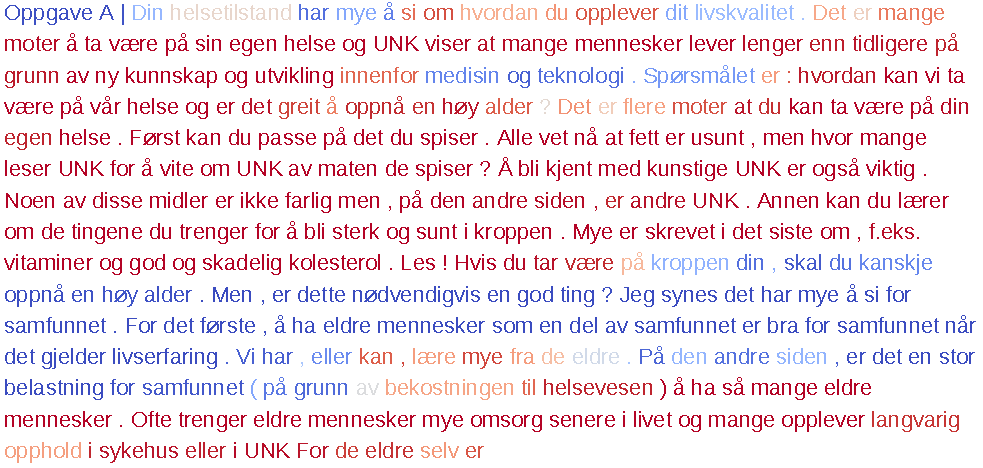
\includegraphics[width=\textwidth]{h0169-eng}
  \caption[Attention in a text by an English speaker]{
    Attention values of NLI classifier on excerpt from ASK text h0189. L1 is
    English, CEFR score B2.
  }
  \label{fig:eng-attention}
\end{figure}

\begin{figure}
  \centering
  
\includegraphics[width=\textwidth]{h0185-rus}
  \caption[Attention in a text by a Russian speaker]{
    Attention values of NLI classifier on excerpt from ASK text h0186. L1 is
    Russian, CEFR score B1/B2.
  }
  \label{fig:rus-attention}
\end{figure}

The Russian speaker's text (fig. \ref{fig:rus-attention}) is almost entirely
high-attention in this excerpt. There is a section of low-attention, around
three sentences long, in the middle of the excerpt. We can therefore not pick
out specific features that the model seems to focus on.

One of the findings in \textcite{pepper2012} was that speakers of Slavic
languages tend to use fewer indefinite articles. In this excerpt we see an
example of the opposite, for instance in the twice occurring `*en god helse'
(\emph{*a good health}). `Helse' (\emph{{health}}) is an uncountable noun,
and should therefore not have an indefinite article, neither in Norwegian nor
English. While this runs counter to the general trend for learners with
Slavic \acp{L1}, it could perhaps be interpreted as a case of
hypercorrection, i.e. a conscious effort to use articles that results in
false positives.

\begin{figure}
  \centering
  
\includegraphics[width=\textwidth]{s0546-som}
  \caption[Attention in a text by a Somali speaker]{
    Attention values of NLI classifier on full ASK text s0621. L1 is Somali,
    CEFR score A2.
  }
  \label{fig:som-attention}
\end{figure}

In the Somali speaker's text (fig. \ref{fig:som-attention}), most of the text
has low attention, except for shorter segments with high attention. However,
the attention is not highest on the most obvious mistakes.

In \textcite{pepper2012}, Somali speakers were found to use the auxiliary
`skal' (\emph{shall/will}) and the pronoun `jeg' (\emph{I}) more frequently
than native Norwegian speakers and several other L1 groups.
\citeauthor{pepper2012} suggested that the frequency of `skal' partly might
be explained by topic bias, since some essay prompts were about the future,
and `skal' is often involved with the future tense. This excerpt is not one of
these texts, and concerns a past experience. Thus, it is not surprising that
it contains no occurrences of `skal'. On the other hand, `jeg' is indeed a
frequent word, occurring five times in the course of a rather short text.

\begin{figure}
  \centering
  
\includegraphics[width=\textwidth]{s0628-vie}
  \caption[Attention in a text by a Vietnamese speaker]{
    Attention values of NLI classifier on excerpt from ASK text s0180. L1 is
    Vietnamese, CEFR score B1/B2
  }
  \label{fig:vie-attention}
\end{figure}

In the Vietnamese speaker's text (fig. \ref{fig:vie-attention}), the word
Vietnam appears three times. This should be a very informative word, as it is
likely that when someone mentions a country in this context, it is their
country of origin. Two of the occurrences have low attention, and one (on the
second-to-last line) has high attention. Within the high-attention segments, we
find a couple of places were the V2 word order in Norwegian shows up. In one
case, `Da jeg var bare ti år` (\emph{Then I was only ten}), the learner gets
the word order wrong (`jeg' and `var' should switch places), but in another
case, `I Vietnam må du ta en [...] prøve' (\emph{In Vietnam you have to take
a test}), they correctly apply V2 word order.


\subsection{Latent space}

We can use dimensionality reduction methods such as $t$-SNE or \ac{PCA} in
order to see if the intermediate representation of documents prior to the
final classification layer positions documents that should be similar close
to each other. In figure \ref{fig:pca-rnn-cefr} we have taken the documents
in the dev set and computed these representations using a BiGRU, then run
them through the PCA algorithm in order to reduce them to two dimensions. The
dimensions are the two axes that account for most of the variance in the
data, and they are orthogonal to each other.

\begin{figure}
  \centering
  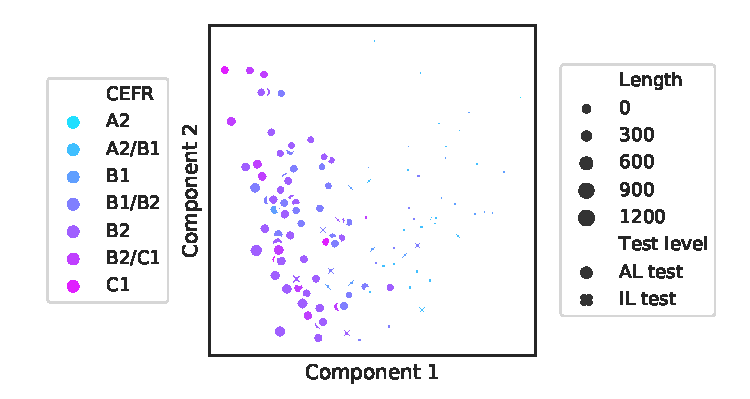
\includegraphics{pca-rnn-cefr}
  \caption[PCA plot of the vector representations of documents]{
    Each document in the dev set is plotted according to its two principal
    components after PCA dimensionality reduction. Marker size and style
    corresponds to document length and test level, respectively.
  }
  \label{fig:pca-rnn-cefr}
\end{figure}

We see that the first component maps closely to the length of the document.
As previously discussed, there is correlation between the length of essays
and the proficiency score, as well as the test level (IL level or AL level).
The PCA plots demonstrates that this relationship is preserved after the RNN
transformation of a document into a feature vector.
